\documentclass{article}

\usepackage{graphicx}
\usepackage{epigraph}
\usepackage[nottoc,numbib]{tocbibind}

\title{Effect Network \\ \LARGE{Decentralized Network for Artificial Intelligence} \\ \vspace{24pt} \Large DRAFT}
\date{November 1, 2017}
\author{Jesse Eisses, Laurens Verspeek, Chris Dawe \\
  \small \texttt{\{jeisses, lverspeek, cdawe\}@effect.ai}}

\makeatletter         
\def\@maketitle{
  \begin{center}
    {\Huge \bfseries \sffamily \@title }\\[4ex] 
    {\Large  \@author}\\[4ex] 
    \@date\\[6ex]
    \includegraphics[width=35mm]{pictures/logo-effect.png}\\[6ex]
  \end{center}}
\makeatother

\begin{document}

\maketitle
\thispagestyle{empty}

\begin{abstract}
  The Artificial Intelligence market is growing at a remarkable rate
  but has become more inaccessible than ever. The requirement for large 
  annotated datasets and a complex technical infrastructure has driven AI 
  development behind the closed doors of corporations. This paper 
  introduces an open, decentralized network called
  \emph{Effect}, that provides services in the Artificial Intelligence
  market. The network replaces several existing services and requires
  no fees, has a low barrier of entry and provides fast growth of the industry. 
  This is accomplished by three platforms that run on the NEO~\cite{neo}
  blockchain and are fueled by a network token called AIX. The first
  platform is a marketplace for tasks that require human
  intelligence. It allows anyone in the world 
  to perform tasks for a fair payment and gives businesses access
  to a large workforce of human intelligence. The second platform is a
  decentralized registry of AI services described by a rich
  ontology. On this platform any algorithm can be accessed as a 
  service in a unified manner and has a convenient way to receive payment. The last
  platform provides a decentralized, distributed computational
  platform that can run popular deep learning frameworks.
  The effect of this network will define the future relationship between humans and AI.
\end{abstract}
\nonumber
\newpage

\tableofcontents
\newpage

\epigraph{\textit{Whether we are based on carbon or on silicon makes
    no fundamental difference; we should each be treated with
    appropriate respect.}}{Arthur C. Clarke}

\section{Introduction}
In the past five years there has been a rapid growth in the number of
practical Artificial Intelligence (AI) applications around us. Smart
services, like self-driving cars, face and voice recognition in mobile
phones and image translation are getting a central place in everyday
life. This rise can be explained by the advances in machine learning
research and the ready availability of cloud computing. This has
resulted in large adoption by the industry and the birth of a
billion-dollar-economy around smart applications. While academic achievements are
available to the public, most intelligent algorithms are developed
behind the closed doors of large corporations. We propose a
private, decentralized ecosystem called the \emph{Effect Network}. The
network is designed to provide a feature complete alternative to the
services shown in Table~\ref{tab:service_compare}, and operates fully
on smart contracts deployed on a Turing-complete blockchain.

\begin{table}[htb]
  \centering
  \begin{tabular}[h]{l|l|l}
    \textbf{Market} & \textbf{Suppliers} & \textbf{Market Cap.} \\ \hline
    Micro tasking & Amazone Mechanical Turk, Fiverr & \dots \\ 
    AI as a service & IBM Watson, Amazon Rekognition & \dots \\
    ML Computation & Google Cloud ML, Amazone AI & \dots 
  \end{tabular}
  \caption{Overview of markets (WIP)}\label{tab:service_compare}
\end{table}

\subsection{Blockchain}
A blockchain is a decentralized data store that can contain arbitrary
logic and processes, without the need for a trusted central
party. Blockchain was first proposed in the Bitcoin whitepaper by
Satoshi Nakamoto, 2009~\cite{nakamoto2008bitcoin}. Since then the technology
has been applied in many areas, and has had a disruptive
influence in the markets of banking, insurance, real-estate and many
more. Decentralized applications have some unique properties like
transparency and a fixed history. We propose a protocol that
decentralizes the global market in Artificial Intelligence; which
lowers the barrier for entry, stimulates market growth and greatly
reduces usage cost.

\subsection{Artificial Intelligence Market}
The AI market will benefit from decentralization because of the high
degree of interaction between agents. An open and decentralized ledger 
can facilitate the interactions and will boost collaboration between parties.
The main reasons that currently make AI development
inaccessible for individuals are listed below:

\begin{description}
\item[Data processing] Intelligent applications perform tasks that
  traditionally require human feedback. Such tasks involve processing
  unstructured data and finding patterns that can provide useful
  output. These applications are trained on large data sets with
  annotations. Obtaining an annotated data set is non-trivial and
  requires a lot of time and money.
  
\item[Diverging tasks] An obstacle when developing a complex
  algorithm is the need to interact with parts of the world outside
  the current domain. For example: a self-driving car learning to steer 
  will also need to identify road signs around the world. This
  situation can best be treated as a knowledge system where the
  classification of the sign is done by an external application. This
  quickly increases the amount of work needed.
  
\item[Computational cost] Developing and training a large AI is a
  computational intensive task. This requires a technical
  infrastructure capable of processing terabytes of data, doing
  batched processing on multiple GPUs and coordinating the
  results.
\end{description}

These three points are solved by the \emph{Effect Network}. Like other
decentralized applications, \emph{Effect} directly connects supply and
demand without the need for an intermediary party. This brings many
advantages:

\begin{itemize}
\item \textbf{Accessibility.} By directly linking supply and demand
  through our micro-tasking platform (see section \ref{sec:phase1})
  \emph{Effect Mechanical Turk} will make training AI algorithms easier,
  faster and cheaper. This will enable users who do not have access to
  a large dataset or a big network to train their AI algorithm.
\item \textbf{Accuracy.} The \emph{Effect Exchange} is an exchange with
  a rich ontology of specialist AI applications. Individual
  applications are able to find each other to buy or sell information, as
  specified in section \ref{sec:phase2}. Through this exchange, users
  can use data sets with significantly higher complexities to train
  their AI algorithms.
\item \textbf{Performance.} Users can directly buy existing data sets
  on the \emph{Effect Exchange} (section \ref{sec:phase2}) or quickly
  create their own data set by creating micro-tasks on the \emph{Effect
    Mechanical Turk} platform (section \ref{sec:phase1}). By enabling
  users to retrieve accurate data sets quickly, they can immediately
  use these datasets to train AI Algorithms.
\item \textbf{Interoperability.} By putting the AI algorithms on the
  blockchain and creating a standard to which these AI algorithms have
  to comply to, we can truly decentralize AI and achieve
  interoperability between individual AIs. The combination of multiple
  AI algorithms will result in powerful capabilities and emergent
  intelligence that no single AI algorithm can achieve on his own.
\end{itemize}

The network will be deployed in consecutive phases, allowing adaption
and development of the network to grow together. The phases cover
independent market sections but are interconnected in our network model
and are all fueled by the same token, called \emph{AIX}.

\section{Phase 1: Decentralized Mechanical Turk}
\label{sec:phase1}
The \emph{Effect Mechanical Turk} platform is a decentralized, peer to
peer marketplace for tasks that require human intelligence.  It
provides similar features as centralized services like Amazon
Mechanical Turk\footnote{https://www.mturk.com}, Fiverr\footnote{https://www.fiverr.com},
Crowdsource\footnote{https://www.crowdsource.com} and Guru.com\footnote{https://www.guru.com}. It is a crowd sourcing
technology that enables requesters to submit tasks that can be
completed by human agents in exchange for compensation. Users can work
on tasks from requesters at any time, anywhere and from any
device. The tasks are called Human Intelligence Tasks (HIT). The
providers of the HIT’s are called \emph{requesters} (see section \ref{subsec:requesters}). When a worker
completes a task they are paid with the cryptographic token AIX.

\begin{figure}[htb]
  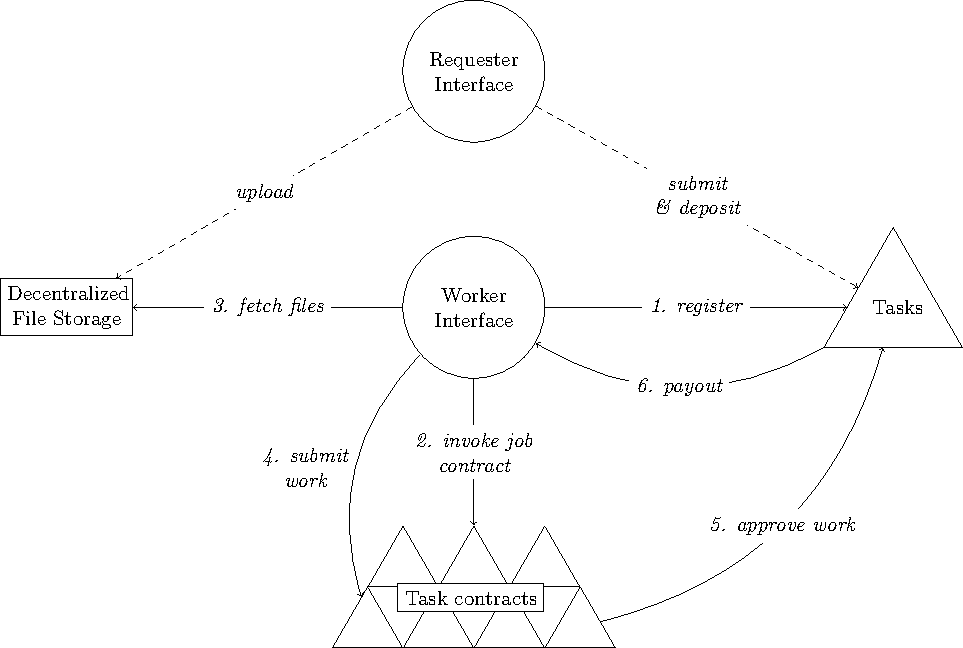
\includegraphics[width=\textwidth]{pictures/emt.pdf}
  \caption{Process of submitting tasks on the \emph{Effect Mechanical Turk}}
\end{figure}

\subsection{Requesters}
\label{subsec:requesters}
\emph{Effect Requesters} can put tasks (see section
\ref{subsec:tasks}) on the \emph{Effect Mechanical Turk} platform to
be completed by workers. The requesters can decide how many AIX the
workers will get for each completed task. The requesters can retrieve
the results from the \emph{Effect Mechanical Turk} platform and use
these results to, for example, train their AI algorithm. \emph{Effect
  Mechanical Turk} gives requesters access to an on-demand, scalable
and distributed workforce.

\subsection{Workers}
\emph{Effect Workers} can complete the tasks from the requesters in
exchange for the AIX tied to these tasks (see section
\ref{subsec:tasks}).

\subsection{Tasks}
\label{subsec:tasks}
A task represent a piece of work that has been submitted by a requester, 
and can be accepted by workers that match its requirements.
Each task points to a data set that can contain any amount of media
assets. The contract ID of the task will validate the format of the
data. Extracting and presenting examples from the data set is done by
the user interface.

A task has at least the following properties:

\begin{table}[h]
  \centering
  \begin{tabular}[h]{r|l}
    Data set & URL \\
    Description & description of the task \\ 
    Contract ID & smart contract that will handle task \\
    Blueprint & data for the contract \\ 
    Required \emph{honor} & require trusted users \\
    Reward & rewarded AIX upon completion \\
    Num. ratings & number of ratings per user \\
    Rating timeout & timeout on performing a rating \\ 
    Expiration  & block ID after which task expires \\
    Sequence id & for sequencing examples (optional)\\
    Data credentials & to unlock private data sets \\
  \end{tabular}
  \caption{Properties of a task}
  \label{tab:task}
\end{table}

The structure and required feedback for a task is defined by the
contract ID and the blueprint. Each type op task requires a smart
contract to handle interaction. \emph{Effect} maintains a database 
of deployed
smart contracts to make it easy for requesters and workers to interact
with the network. Adding smart contracts to the network is handled
through governance (section~\ref{sec:governance}). Affiliate programs
will cover costs of deploying new contract types. 

\subsection{Data sets}
Data sets are often large and consist of various types of media. A
blockchain is not a suitable database for storing this kind of
information. Other decentralized storage options, like
BitTorrent\footnote{http://www.bittorrent.com} and IPFS\footnote{https://ipfs.io}, are specialized in these
types of assets. For this reason the network will use such a
hash-based distributed file storage, where each media asset can be
referred to by a single hash.

Note that the feedback on a \emph{task} can also involve storing media
assets, for example in tasks like image segmentation. In this case the
ratings asset will be stored on the distributed storage, and a hash
and checksum of the rating are stored on the blockchain.

Requesters will also be able to supply data sets through traditional
channels, like Amazon S3, Google Cloud Storage and FTP.

\subsection{Privacy}
The blockchain is decentralized and open by nature. These properties
are not always desirable, for example when privacy is concerned. 
There are several
measures that must be taken to make sure the Effect network can be
used for sensitive information. The network can provide privacy for
the following cases:

\begin{description}
\item[Datasets] Requesters can provide their data set in encrypted
  form. Only selected users will be able to decrypt or access the
  data. This is determined by network smart contracts using Public Key
  Encryption, where selected users can decrypt the data set
  credentials.
\item[User ratings] Ratings of tasks performed by workers are stored
  on the blockchain, using Public Key Encryption. The public key of
  the owner is used to sign the ratings, so only the owner of the task
  can view the ratings.
\end{description}

Tasks that involve privacy features will be more computational
expensive, thus will also have a higher network fee.

\newpage
\epigraph{\textit{I believe that at the end of the century the use of words and general educated opinion will have altered so much that one will be able to speak of machines thinking without expecting to be contradicted.}}{Alan Turing} 
\section{Phase 2: Decentralized AI Exchange}
\label{sec:phase2}

The \emph{Effect Exchange} is a decentralized marketplace where
AI algorithms can exchange their services. An application owner can
register on the exchange by specifying a public endpoint of his
application, following our data interchange format and specifying a
usage fee for consumers. This application can now be invoked through
smart contracts on the blockchain. The caller of the contract will
have to transfer the required funds to the owner of the contract to
get an authorization token that allows him to interact with the application.

Thanks to the application registry, algorithms are able to explore
possible collaborations over the blockchain. It also encourages
standardization of data exchange formats, as interoperability with
other applications means more interactions: a financial incentive.

\subsection{Application registry}
The network will maintain a registry of available applications. This
registry will be enriched with a semantic ontology that describes the
application, as well as a technical schema of its inputs and
outputs.

\subsection{Endpoints}
Application endpoints on the \emph{Effect AI Exchange} communicate
over the HTTP protocol. Data is exchanged in JSON format and should
strongly confirm the defined RDF schema.

Requests signed with the private key of the buyer will be accepted by
the endpoint. Issuing authorization tokens and checking their validity
can be done by public APIs that hold a partial index of the
blockchain. They could request small fees for providing this service.


\section{Phase 3: Decentralized AI Algorithms}
\label{sec:phase3}
Phase 1 and 2 of the \emph{Effect} network decentralized the data
gathering and usage of AI algorithms. Up to this point the algorithms
themselves still run on centralized servers. In the final phase of the
network the actual computation will be distributed, so that the
algorithms run globally without a single point of failure. To achieve
this we use the fact that most machine learning algorithms have rigid
structure, and operate on sets of weights. These types of algorithms
are relatively easy to distribute. The \emph{Effect} decentralized
compute engine is based on popular deep-learning networks like
\emph{Caffe}, \emph{MXNet} and \emph{Tensorflow}, where the network
structure can be defined as a declarative graph and weights are stored as
matrices of real numbers. These matrices can be distributed over a decentralized
file system and be processed at different compute nodes on the network.

\section{Community}
The described network can be deployed and used as a decentralized
application as-is. However, in order for the network to grow and be
sustainable, we believe there has to be a form of governance. Parties
should have incentive to use the AIX token for the purpose of AI
tasks. Investors looking for quick monetary gain should be discouraged
and pump-and-dump schemes should be avoided, in order for the network
to grow and slowly take market value from the existing centralized
services.

\subsection{AIX and the Galaxy Pool}
It is important to maintain liquidity in AIX, especially during the
early days when there is no listing on exchanges. Ideally the
following actions should always be possible:

\begin{enumerate}
\item Workers are able to sell their AIX rewards for native tokens
\item Requesters and network users should be able to buy AIX
\end{enumerate}

For a new token on the market this kind of liquidity can be hard to
achieve and can be hurt by speculative trading.

The Effect Network will maintain a central pool of tokens to provide
liquidity, encourage adoption and stabilize network fees. This pool is
called the Galaxy Pool and consists of a mix of AIX and native
tokens. Several rules will drive the Galaxy Pool towards an
equilibrium. These rules can later be refined by means of
governance as is discussed in section~\ref{sec:governance}.

\begin{figure}[htb]
  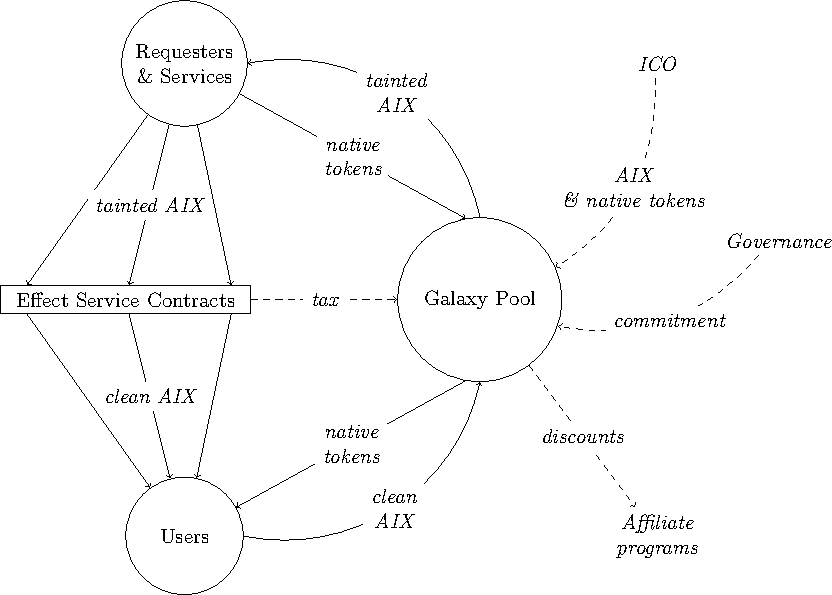
\includegraphics[width=\textwidth]{pictures/galaxy.pdf}
  \caption{Diagram of the \emph{Effect} governance model and
    construction of the Galaxy Pool}
\end{figure}

The Galaxy Pool ensures stable exchange rates for users of the
platform at all times. The pool is not suitable for day traders, as
only \emph{tainted} coins can be bought. Any coin that is bought from
the Galaxy will initially be tainted, and a tainted coin can not be
sold back to the pool. A tainted coin is \emph{washed} (converted to a
regular AIX token) by spending it through an \emph{Effect} service
contract. These are the service contracts from the tasks and service
registry. This protects the Galaxy Pool from external manipulation and
keeps exchange rates stable for workers.

\subsubsection{Proof of Commitment}
\label{subsec:commitment}
- \emph{In conceptual development} -

\subsection{Honor Tokens and Fraud}
On the \emph{Effect Mechanical Turk} workers are rewarded tokens for
their effort. This could make malevolent users to gain wealth by
submitting a large quantity of tasks with poor quality. To avoid this,
the network will appraise users by their quality of work. Users that
put in good effort will be rewarded with \emph{Honor Tokens} (HNR). These
tokens can not be traded or sold, but will gradually expire over
time. Workers with a large number of honor tokens will be able to
apply for more high rewarding tasks and will have to pay less tax to the
Galaxy Pool.

HNR tokens are credited to users ad-hoc when they are rated for good
work. There are 2 ways this can happen:

\begin{enumerate}
\item The task owner can add ground-truth ratings of examples. If a
  worker rates an example with a ground-truth similar to the ground
  truth, they are rewarded 1 HNR, else they loose 1 HNR. Ground-truth
  examples are stored encrypted on the blockchain and the decryption
  key is shared by the requester after the task has expired. Thus the
  rating takes place after task expiration time.
\item Workers that give similar ratings on the same HIT are credited
  with 1 HNR. This is done periodically and at random. Workers that
  consequently give deviant feedback are subtracted HNR.
\end{enumerate}

\subsection{Governance}
\label{sec:governance}

The blockchain is immutable by nature so the network needs a way to
apply changes to its components. There are 2 types of changes that can
be applied. First are the variables defined in smart contracts that
can change over time, for example the exchange rates in the Galaxy
Pool and the tax over service transactions. The second are the smart
contracts themselves; introducing new service contracts - like new
task types - and amending existing contracts will be necessary in the 
future. As the \emph{Effect Network} is 
decentralized there can not be a single person or organization 
authoring  these changes. To fix this the network has a governance 
system that allows prominent people in the community to propose and
vote for improvements, as explained in~\ref{subsec:improvments}. Right 
to vote is at first acquired by selected individuals as discussed in
\ref{subsec:counsel}.

\subsection{Improvement Proposals}
\label{subsec:improvments}
Both smart contracts and service variable adjustments should be submitted 
to an improvement proposal system. Each proposal contains logic for adjusting 
parts of the ecosystem. A proposal is only executed if a majority of the
council members voted in favor of it within a time limit.

\subsection{Council}
\label{subsec:counsel}
The \emph{Effect Council} is an group of 51 individuals that are allowed to 
cast a vote on improvement proposals.

\section{Implementation}

This section contains examples of how the platform would function when
built on the NEO blockchain. NEO is a blockchain that uses Delegate
Byzantine Fault Tolerance (dBFT) consensus and features Turing-complete smart
contracts. It also has features for user identification and file
storage that make it a very suitable host for the \emph{Effect
  Network}.

\subsection{Galaxy Pool: NEO and GAS}
In NEO there are 2 native tokens: \emph{NEO} and \emph{GAS}. The GAS
is a utility token that is used for paying network fees; which are
deploying and executing smart contracts. NEO acts as a share in the
platform; holding NEO gives a payout in GAS from network usage. In
this setup, the Galaxy Pool should hold a combination of AIX, NEO and
GAS to function correctly. The NEO is used to payout workers at a
stable exchange rate and to increase the GAS stake by collecting dividend. As
NEO is indivisible the rate should be defined in
$\frac{AIX}{NEO}$. The GAS is used to pay any network fees to users of
the network, so workers will not have to go to an exchange to use the
platform. The GAS is also used to deploy new smart contracts and amend
existing smart contracts. This is crucial as the \emph{Effect Network}
will be developing all the time.

\newpage
\epigraph{\textit{Control is as much an effect as a cause, and the
    idea that control is something you exert is a real handicap to
    progress}}{Steve Grand}
\section{Conclusion}

Having an open, accessible and affordable platform for intelligent
algorithms to operate and develop will be a key component
in the coming century. Artificial Intelligence and decentralization
are a natural match. Along with the rise of blockchain technology and
the surge in the global AI-market this enables big opportunities. The
\emph{Effect Network} effectively combines the two technologies. It will
replace a significant portion of the $3.1$ trillion USD AI-market by a
decentralized platform, giving immediate practical and monetary
value. It also has the potential of becoming the breeding ground for
emerging AI-technologies and will be at the front of AI emancipation.

Registering AI interactions on the blockchain also has benefits for
society. Bill Gates had the idea to tax labor performed by
AI-algorithms, to compensate for the loss of jobs in many sectors. This
idea seemed science fiction at the time, but this can be realized on the 
\emph{Effect Network}; where algorithms are registered, can control
their own bank account, and have transactions published on the
blockchain.

The long term success of the project will depend on many factors. Most
important is the initial implementation of the concepts described in
this paper, and the performance of the governance model proposed in
section~\ref{sec:governance}. The effect of this network will define the future relationship between humans and AI.

\bibliographystyle{unsrt}
\bibliography{references}

\end{document}